\chapter{Fabrication d'un transistor moléculaire}
Afin de caractériser un aimant moléculaire unique, nous avons décidé de l'intégrer dans un dispositif à trois terminaux, c'est-à-dire, fabriquer un transistor à molécule unique~(SMT - Single Molecule Transistor). Du fait de la petite taille de ces dernières~($1\,nm$ environ), il est impossible de faire appel à des techniques lithographiques classiques. Nous avons déjà abordé les différentes solutions développées dans le cadre de la spintronique. Nous avons fait le choix d'utiliser la technique d'électromigration développé par H. Park \textit{et al.} avec quelques adaptations.

Deux éléments sont prépondérants dans la qualité d'un SMT : l’efficacité de la grille et la bonne qualité des interstices. Nous présenterons dans une première partie les différentes étapes nous permettant d'obtenir une grille efficace, après avoir défini les critères définissant cette efficacité. Ensuite, nous montrerons comment il est possible, en utilisant le phénomène d'électromigration, de produire des interstices nanométriques. Nous verrons enfin la technique de dépôt des molécules ainsi que les premières étapes de caractérisation électrique des dispositifs obtenus.


\begin{figure}
\parbox{6.5cm}{
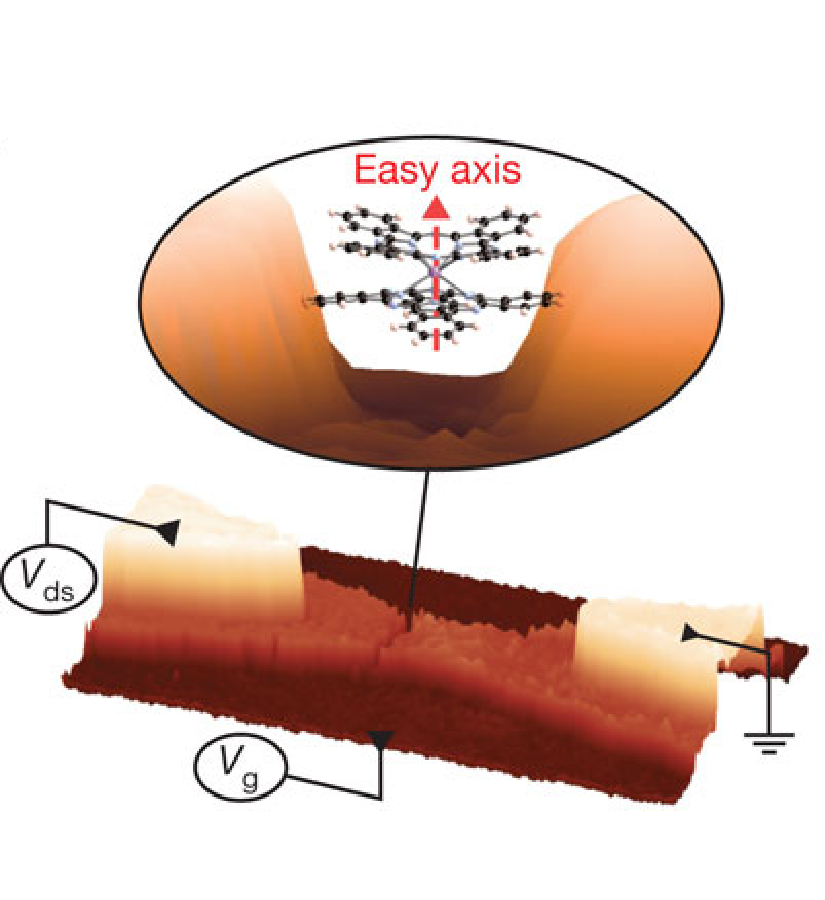
\includegraphics[scale=0.45]{Fabrication/ImageTrans/ImageTrans.pdf} 
}
\parbox{7cm}{\caption{Extrapolation 3D d'une image obtenue par microscopie électronique à balayage. Elle correspond à la structure finale que l'on souhaite obtenir : les électrodes de source et de drain, l'électrode de grille, ainsi qu'un interstice nanométrique dans lequel une molécule est piégée~(extrait de~\cite{Vincent2012}).}
\label{ImageTrans}
}
\end{figure}

\section{Réalisation d'une grille locale}
La grille est un élément essentiel du transistor et c'est également vrai d'un transistor moléculaire~\cite{Datta2009,Zant2006}. Dans ce dernier cas, elle permet notamment de moduler le potentiel chimique de la molécule allant jusqu'à modifier son état de charge~\cite{Beenakker1991,Wiel2002,Hanson2007}~(cf annexe sur le transport mésoscopique). Elle permet également de contrôler la conductance du système~(avec le concours de la tension source-drain), et donc de choisir des points de fonctionnement adaptés. Nous détaillerons ce dernier point dans le chapitre résultat. 

L'efficacité intrinsèque d'une grille peut être résumée en un seul critère~:~la charge induite. Celle-ci s'exprime simplement par $Q = CV_g^{max}$ où $Q$ est le charge induite et $C$ est la capacité associée à la grille, $V_g^{max}$ étant la tension maximale applicable à la grille. Elle dépend essentiellement de trois paramètres physiques : le champ électrique maximum applicable, l'épaisseur et la permittivité de l'oxyde~\cite{Biercuk2003}. 

Outre les paramètres que l'on vient de voir, il existe plusieurs géométries de grille susceptibles d'avoir une influence sur l’efficacité de cette dernière. On peut identifier trois géométries : la grille au-dessus ou  ``\textit{top-gate}'', la grille latérale et la grille arrière ou  ``\textit{back-gate}''.

\subsection{Les différentes géométries}
Je ne donnerai ici qu'une rapide présentation des différentes grilles existantes. Une comparaison plus détaillée entre ces différentes géométries est disponible dans la thèse d'Aurore Mangin~\cite{Aurore2009}.

\begin{figure}
\centering 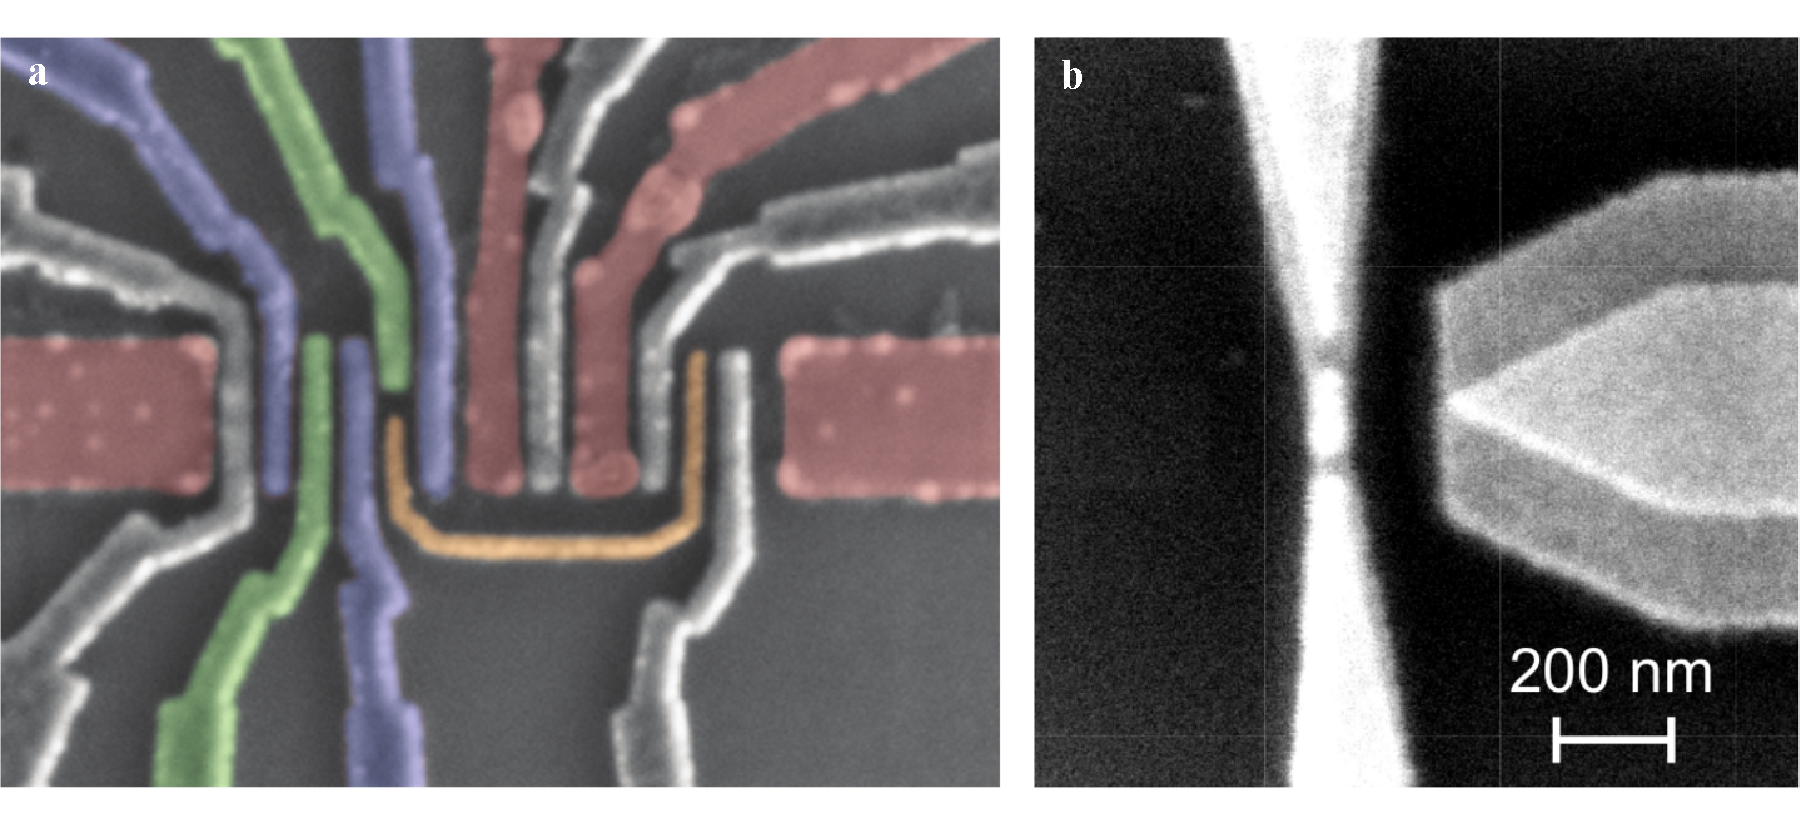
\includegraphics[scale=0.45]{Fabrication/Gateconf/GateConf.pdf}
\caption{Images obtenues par microscopie électronique à balayage. \textbf{a} : nanotube sur lequel on est venu positionner 9 grilles afin de réaliser un double point quantique ainsi qu'un détecteur de charge ~(extrait de \cite{Churchill2009}). \textbf{b} : configuration en grille latérale réalisée dans la cadre de jonctions électromigrées~(extrait de~\cite{Aurore2009}).}
\label{GateConf}
\end{figure}


\subsubsection{La ``\textit{top-gate"}}
Cette configuration est utilisée dans le cas des transistors à effet de champ conventionnels. On la retrouve également dans les dispositifs expérimentaux faisant appel à des nanofils~\cite{Fasth2005} ou bien encore à des nanotubes~\cite{Javey2002}~(cf Fig.\ref{GateConf}.\textbf{a}). Elle a également pu être implémentée dans le cas de nanotubes suspendus donnant des résultats plus que convaincants~\cite{Leturcq2009}.

Cette configuration est cependant difficilement compatible avec l'électromigration. En effet, celle-ci est effectuée après les étapes de lithographie, ce qui serait impossible si le fil d'or était recouvert par une grille. Pour produire une grille compatible avec l'électromigration, il faut se tourner vers d'autres géométries comme la configuration latérale.

\subsubsection{La grille latérale}
Cette configuration consiste à placer la grille latéralement vis-à-vis du gap obtenu par électromigration~\cite{Mangin2009}~(cf Fig.\ref{GateConf}.\textbf{b}). Accompagnée d'une grille arrière, elle permet d'avoir deux moyens d'action sur le potentiel chimique de la molécule située dans la gap. 

Il est en revanche très difficile de contr\^oler précisément la position de cette grille, et elle se trouve donc souvent située à plusieurs dizaines de nanomètres du gap. De plus, le r\^ole de l'oxyde est dans ce cas joué par l'air, qui possède une permittivité proche de l'unité. Cette configuration abouti donc, de manière générale, à une grille moins efficace que la configuration grille arrière~\cite{Aurore2009} que nous allons voir maintenant.


\subsubsection{La grille arrière}
Dans cette configuration, la grille se situe sous le dispositif. Elle a notamment été adoptée pour la réalisation du premier transistor à molécule unique~\cite{Park2000}. Elle est bien s\^ur compatible avec l'électromigration et, implémentée en grille locale, elle permet d'obtenir des grilles très efficaces. Pour ces raisons, nous avons choisi d’adopter cette configuration pour nos échantillons. De plus, sa fabrication peut \^etre grandement facilitée par l'utilisation de la technique ALD~(Atomic Layer Deposition - dép\^ot par couche atomique) que nous allons présenter dans la suite.


\subsection{Création de l'électrode de grille}

La première étape de la fabrication de notre grille locale consiste en l'obtention de l'électrode de grille. Compte tenu des tailles caractéristiques de cette dernière, cette électrode peut \^etre obtenue à l'aide d'une lithographie optique ultra-violet profond (DUV - Deep Ultra-Violet). A cette fin, une méthode bicouche LOR3A/UV3 est utilisée en suivant les instructions du Tab.\ref{tab_recette}, avec pour seule différence, l'épaisseur d'or déposée à la seconde étape : $20\,nm$.

\begin{table}
\begin{center}
\begin{tabular}{|p{0.5cm}|p{4cm}|p{4cm}|p{3cm}|}
  \hline
\,& \textbf{étape} & \textbf{procédé} & \textbf{paramètres} \tabularnewline
\hline
1 &  nettoyage du wafer & acétone, ethanol, isopropanol et plasma oxygène (RIE)& $2\,$min \tabularnewline
\hline
 2 & étalement de LOR 3A pour une épaisseur de $400\,$nm& tournette & v\,:\,$2000\,$tr.min$^{-1}$, a\,:\,$2000\,$tr.min$^{-2}$, t\,:\,$30\,$s \tabularnewline
\hline
 3 & recuit & plaque chauffante & $1\,$min à $170\,\degres$C \tabularnewline
\hline
4 & étalement de UV3 & tournette & v\,:\,$4000\,$tr.min$^{-1}$, a\,:\,$2000\,$tr.min$^{-2}$, t\,:\,$30\,$s \tabularnewline
\hline
5 & recuit & plaque chauffante & $1\,$min à $130\,\degres$C \tabularnewline
\hline
6 & insolation & aligneur dUV MJB3 & $5.5\,$s à $0.3\,$mW.cm$^{-2}$\tabularnewline
\hline
7 & recuisson & plaque chauffante & $1\,$min à $130\,\degres$C \tabularnewline
\hline
8 & développement & MF-CD-26 & $30-40\,$s\tabularnewline
\hline
9 & neutralisation du développeur & eau DI & $1\,$min\tabularnewline
\hline
10 & dépôt de la couche d'accroche métallique & évaporateur à canon à électron PLASSYS & $5\,$nm de Ti à $0.1\,$nm.s$^{-1}$ \tabularnewline
\hline
11 & dépôt de la couche métallique principale & évaporateur à canon à électron PLASSYS & $80\,$nm de Au à $0.1\,$nm.s$^{-1}$ \tabularnewline
\hline
12 & \textit{lift-off} & acétone & $10\,$min à $1\,$h, on peut l'assister par ultra-son à $80\%$ de la puissance maximum. \tabularnewline
\hline
 13 & dissolution de LOR3A & PG-Remover & $1\,$h à $80\,\degres$C \tabularnewline
\hline
14 & rinçage & acétone et isopropanol & $1\,$min de chaque sous la pissette\tabularnewline
\hline
15 & séchage & azote sec & wafer posé sur du papier absorbant, pistolet à la verticale du wafer, ne pas toucher le wafer avec des pinces\tabularnewline
\hline
16 & nettoyage & plasma oxygène (RIE)& $10\,$min\tabularnewline
\hline
\end{tabular}
\caption{Recette du bicouche LOR3A/UV3 : celle-ci permet de ne plus avoir d'effet de bord lors des \textit{lift-offs}.}
\label{tab_recette}
\end{center}
\end{table}


Cette étape permet également d'obtenir les marques d'alignements nécessaires à la fabrication des lignes d'amenés. Une première série de marques~(cf carré bleu de la Fig.\ref{FinalResult}.\textbf{a}) permet d'effectuer un alignement grossier. Ce dernier est ensuite affiné à l'aide d'une deuxième série de repères~(cf carré vert de la Fig.\ref{FinalResult}.\textbf{a}).

La technique bicouche a été préférée à la technique usuelle monocouche, car elle a l'avantage de prévenir la formation de bords lors de l'étape de lift-off~(cf Fig.\ref{lift-off}). En effet, la présence de ces bords pourrait entraîner une perte de contact entre la jonction et le plot correspondant, lors du passage de marche~(i.e. lorsque la ligne d'amené, réalisée par lithographie électronique, passe de la surface de silicium à la grille, la hauteur de marche étant donnée par l'épaisseur de la grille).


\begin{figure}
\centering 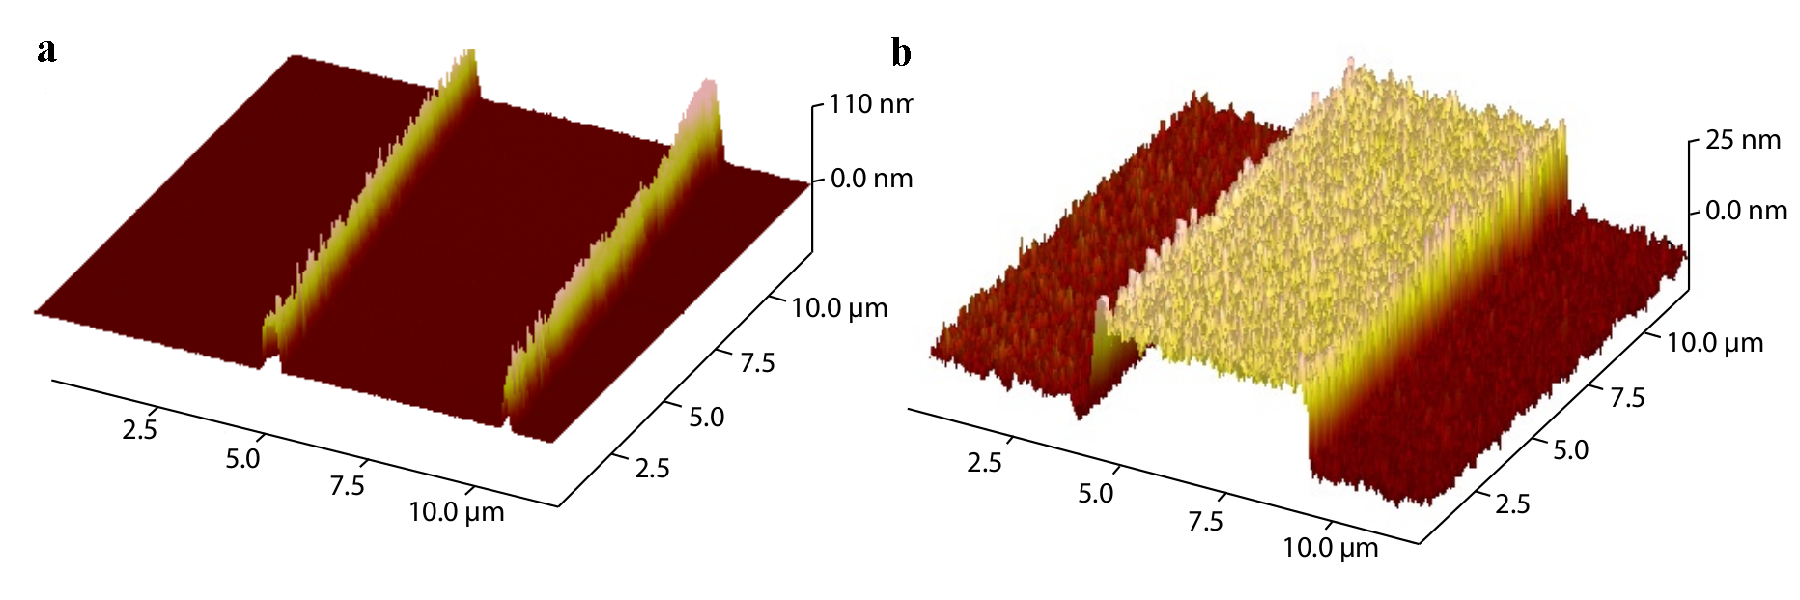
\includegraphics[scale=0.45]{Fabrication/BatmanGrille/BatmanGrille.pdf}
\caption{\textbf{a} : image AFM d'une électrode de grille présentant des bords trop relevés d\^u fait d'un problème de lift-off, obtenue par une technique monocouche. \textbf{b} : image AFM montrant une électrode de grille après lift-off ne présentant pas d'anomalie après lift-off obtenue par la la technique bicouche~(extrait de~\cite{RochPhD}).}
\label{lift-off}
\end{figure}

Cette première étape est suivie du dépôt d'oxyde par une méthode de dépôt par couche atomique ou ALD~(Atomic Layer Déposition) que nous allons détailler maintenant.

\subsection{Le dép\^ot par ALD}

Comme nous l'avons déjà précisé en introduction, le choix de l'oxyde est très important et, en particulier, la permittivité de ce dernier doit être la plus élevée possible.

Parmi les oxydes à haute permittivité, les plus couramment utilisés sont l'alumine~($\kappa \sim 8$), l'hafnia~($\kappa \sim 17$) et l'oxyde de zirconium~($\kappa \sim 26$)~\cite{Biercuk2003}. De manière générale, le premier est obtenu par dépôt d'une électrode d'aluminium, puis exposition à une atmosphère riche en oxygène, ou bien par ALD. Les deux derniers sont en général obtenus par ALD ou, plus rarement, par MOCVD~(Metalorganic Chemical Vapour Deposition). Lorsque je suis arrivé en thèse, la technique par oxydation naturelle était en usage. Bien que relativement facile à mettre en œuvre, il est difficile de connaître avec exactitude l'épaisseur d'oxyde. De plus, nous avons observé une grande variabilité dans la qualité des grilles obtenues par ce procédé.

Nous avons donc développé un nouveau procédé inspiré de~\cite{Biercuk2003}, en utilisant une méthode ALD, nous permettant d'obtenir une grille avec un oxyde de $8\,nm$ environ. Parmi les trois oxydes précédemment cités, nous avons choisi l'oxyde d'hafnium. Celui-ci a l'avantage d'être fortement documenté et présente des performances supérieures à l'alumine pour ce qui est de la charge induite~\cite{Biercuk2003}. 

La technique d'ALD originellement appelée ALE~(pour Atomic Layer Epitaxie) a été brevetée dans les années 1970, et remise au goût du jour pour les besoins toujours plus grands de la micro-électronique~\cite{Leskelae2003}. Elle consiste en une succession de deux réactions auto-limitantes, aboutissant à la formation d'un oxyde comme le montre la Fig.\ref{ALD}.

\begin{figure}
\centering 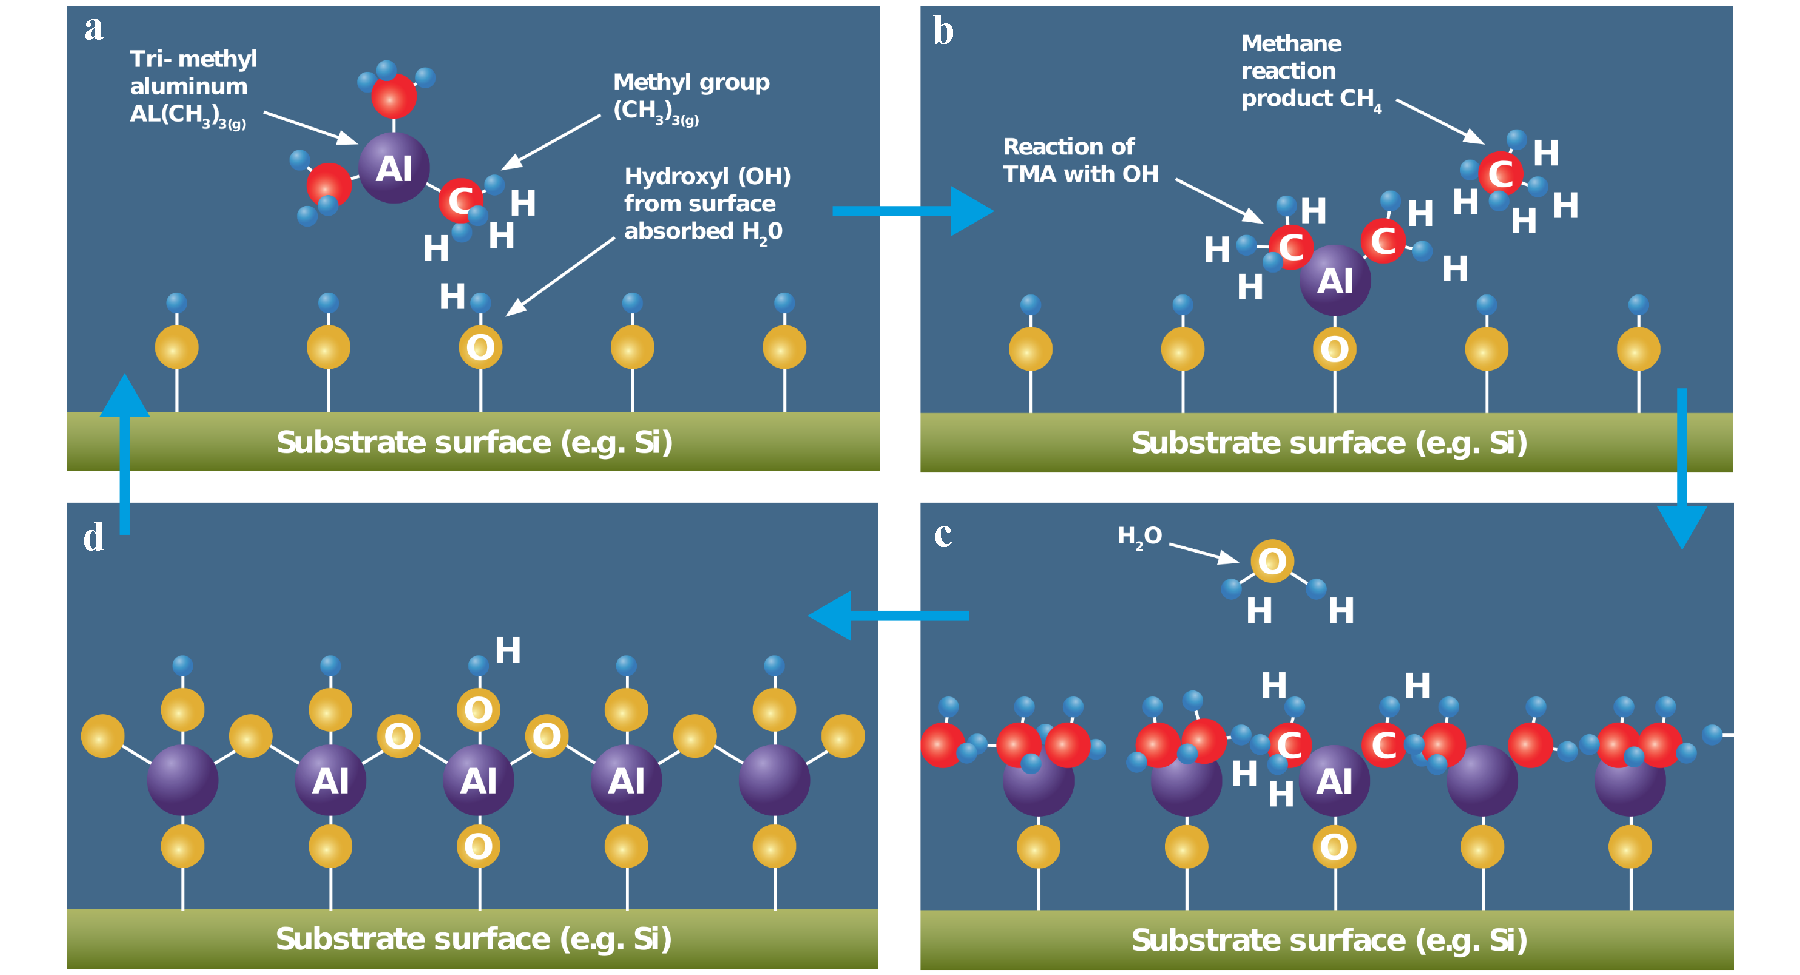
\includegraphics[scale=0.45]{Fabrication/ALD/ALD.pdf}
\caption{Première étape du cycle ALD : le premier précurseur, ici du Al(CH$_3$)$_{3(g)}$, se fixe à la surface~(\textbf{a}) et les produits issues la réaction de fixation sont évacués par un flux de gaz inerte~(\textbf{b}). Dans un deuxième temps, de l'eau est injectée et réagi avec la première couche de précurseur~(\textbf{c}) pour former une couche atomique d'oxyde~(\textbf{d}). Le cycle se répète ensuite à raison d'une couche atomique par cycle. (extrait du site CambrigeNanoTech)}
\label{ALD}
\end{figure}


Le premier avantage de la technique est sa facilité de mise en œuvre. Le contrôle du procédé, couche par couche, permet de choisir l'épaisseur d'oxyde déposée avec une grande précision. De plus, la nature de ce dernier est uniquement déterminée par les précurseurs utilisés, ce qui donne un large choix de matériaux. Afin d'obtenir un oxyde de qualité pour les applications électroniques, celui-ci doit remplir deux critères : il doit contenir peu d'impuretés et être de préférence amorphe~\cite{Kim2003}.

\begin{table}
\begin{center}
\begin{tabular}{|p{0.5cm}|p{6cm}|p{6cm}|}
\hline
\multicolumn{3}{|c|}{\textbf{Réglages}} \tabularnewline
\hline
\multicolumn{2}{|l|}{\textbf{élément}} & \textbf{paramètres} \tabularnewline
\hline
\multicolumn{2}{|l|}{température du précurseur} & $90\, \degres C$ \tabularnewline
\hline
\multicolumn{2}{|l|}{température du \textit{Tee}} & $150\, \degres C$ \tabularnewline
\hline
\multicolumn{2}{|l|}{température de la chambre~(\textit{inner} et \textit{outer})} & $100\, \degres C$ \tabularnewline
\hline
\multicolumn{2}{|l|}{température du \textit{Bellow}} & $150\, \degres C$ \tabularnewline
\hline
\multicolumn{2}{|l|}{\multirow{2}{*}{flux d'azote}} & $20\, sccm$ \newline (pression d'environ $0.5\,Torr$) \tabularnewline
\hline
\hline
\multicolumn{3}{|c|}{\textbf{Procédé}} \tabularnewline
\hline
\,& \textbf{étape} & \textbf{paramètres} \tabularnewline
\hline
1 & impulsion de TDMAH & $0.015\,s$ \tabularnewline
\hline
2 & temps d'attente & $120\,s$ \tabularnewline
\hline
3 & impulsion d'eau & $0.015\,s$ \tabularnewline
\hline
4 & temps d'attente & $120\,s$ \tabularnewline
\hline
\end{tabular}
\caption{Paramètres et réglages du procédé ALD.}
\label{recette_ALD}
\end{center}
\end{table}



Pour remplir le premier critère, il est nécessaire de chauffer de façon suffisante le substrat, afin de désorber efficacement les déchets produits lors de la fixation du précurseur~(cf Fig.\ref{ALD}). Une structure amorphe, au contraire, est obtenue par un dép\^ot à basse température~\cite{Triyoso2004}. Cela a en plus l'avantage de rendre le procédé compatible avec une étape de lithographie~\cite{Biercuk2003}~(évitant une détérioration de la résine) et de diminuer la rugosité de l'oxyde~\cite{Triyoso2004}. Il faut donc arriver à trouver un compromis entre ces deux conditions contradictoires.

Celui-ci a été trouvé en laissant un délai conséquent entre les différentes étapes du dépôt, permettant aux produits de réaction de désorber~\cite{Biercuk2003}. Cela se traduit par un temps d'attente de 2 minutes entre chaque étape de cycle. Un dépôt de 80\,cycles~(environ $8\,nm$) d'hafnia prend donc un peu plus de cinq heures~(pour les détails concernant le dépôt ALD, le lecteur peut se référer au Tab.\ref{recette_ALD}). Si ce temps peut paraître long au premier abord, il ne représente qu'un temps négligeable au regard des autres étapes, et notamment, celle de lithographie électronique que nous allons aborder maintenant.

\begin{figure}
\centering 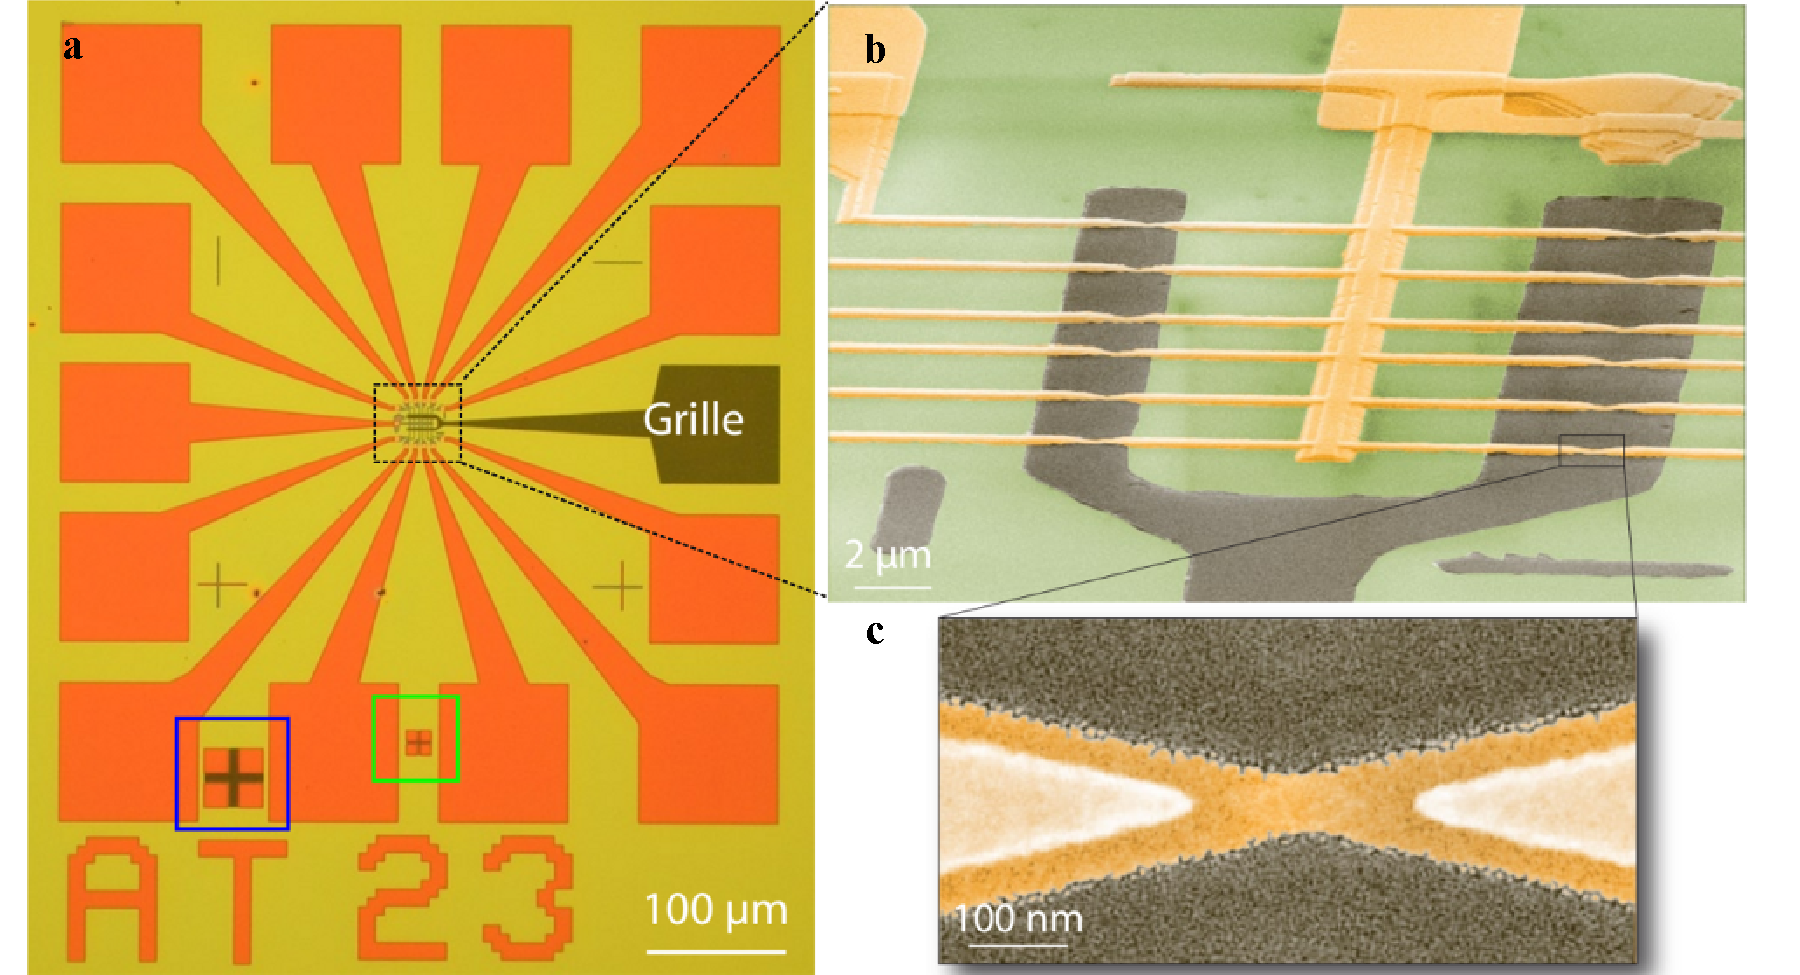
\includegraphics[scale=0.45]{Fabrication/FinalResult/FinalResult.pdf}
\caption{\textbf{a} : Échantillon après les deux étapes de lithographie optique. Les lignes d'amené de courant sont visibles en orange et la grille locale en gris. Les deux carrés repèrent les marques d'alignement. \textbf{b} : Image obtenue par microscopie électronique à balayage montrant la structure centrale de nos échantillons. \textbf{c} : grossissement présentant une constriction obtenue à l'aide de l'évaporation sous angle. La grille, colorée en gris, est clairement visible au centre (extrait de \cite{RochPhD}).}
\label{FinalResult}
\end{figure}


\section{Réalisation d'un nanofil}

Afin de réaliser les nanofils d'or, on procède en deux étapes. Dans la première, une lithographie optique est effectuée afin d'obtenir les plots de connexion. Dans la seconde, une lithographie électronique est réalisée en vue de la fabrication des nanofils.

\subsection{Lithographie optique}

Cette étape de lithographie vise à fabriquer les plots d'or nécessaires à la micro-soudure de notre échantillon, ainsi que les lignes d'amenée de courant~(cf partie orange de la Fig.\ref{FinalResult}.\textbf{a}). La recette du Tab.\ref{tab_recette}  est utilisée pour obtenir un dép\^ot de 80$\,nm$ d'or avec une couche d'accroche en titane.

Le résultat final est présenté dans la Fig.\ref{FinalResult}.\textbf{a} où la partie orange désigne les lignes d'amenée de courant et la partie grise la grille locale. La partie centrale va venir accueillir les nanofils d'or comme nous allons le voir dans la suite.


\subsection{Lithographie électronique}



Comme nous l'avons présenté dans l'introduction, notre méthode de fabrication repose sur la technique d'électromigration. Cette dernière, pour fonctionner correctement, a besoin d'\^etre opérée sur des fils d'or très fins, présentant une section de quelques dizaines de nanomètres, pour une épaisseur de quelques nanomètres en ce qui concerne la partie la plus fine~(cf Fig.\ref{FinalResult}.\textbf{c}). 

\begin{figure}[h!]
\centering 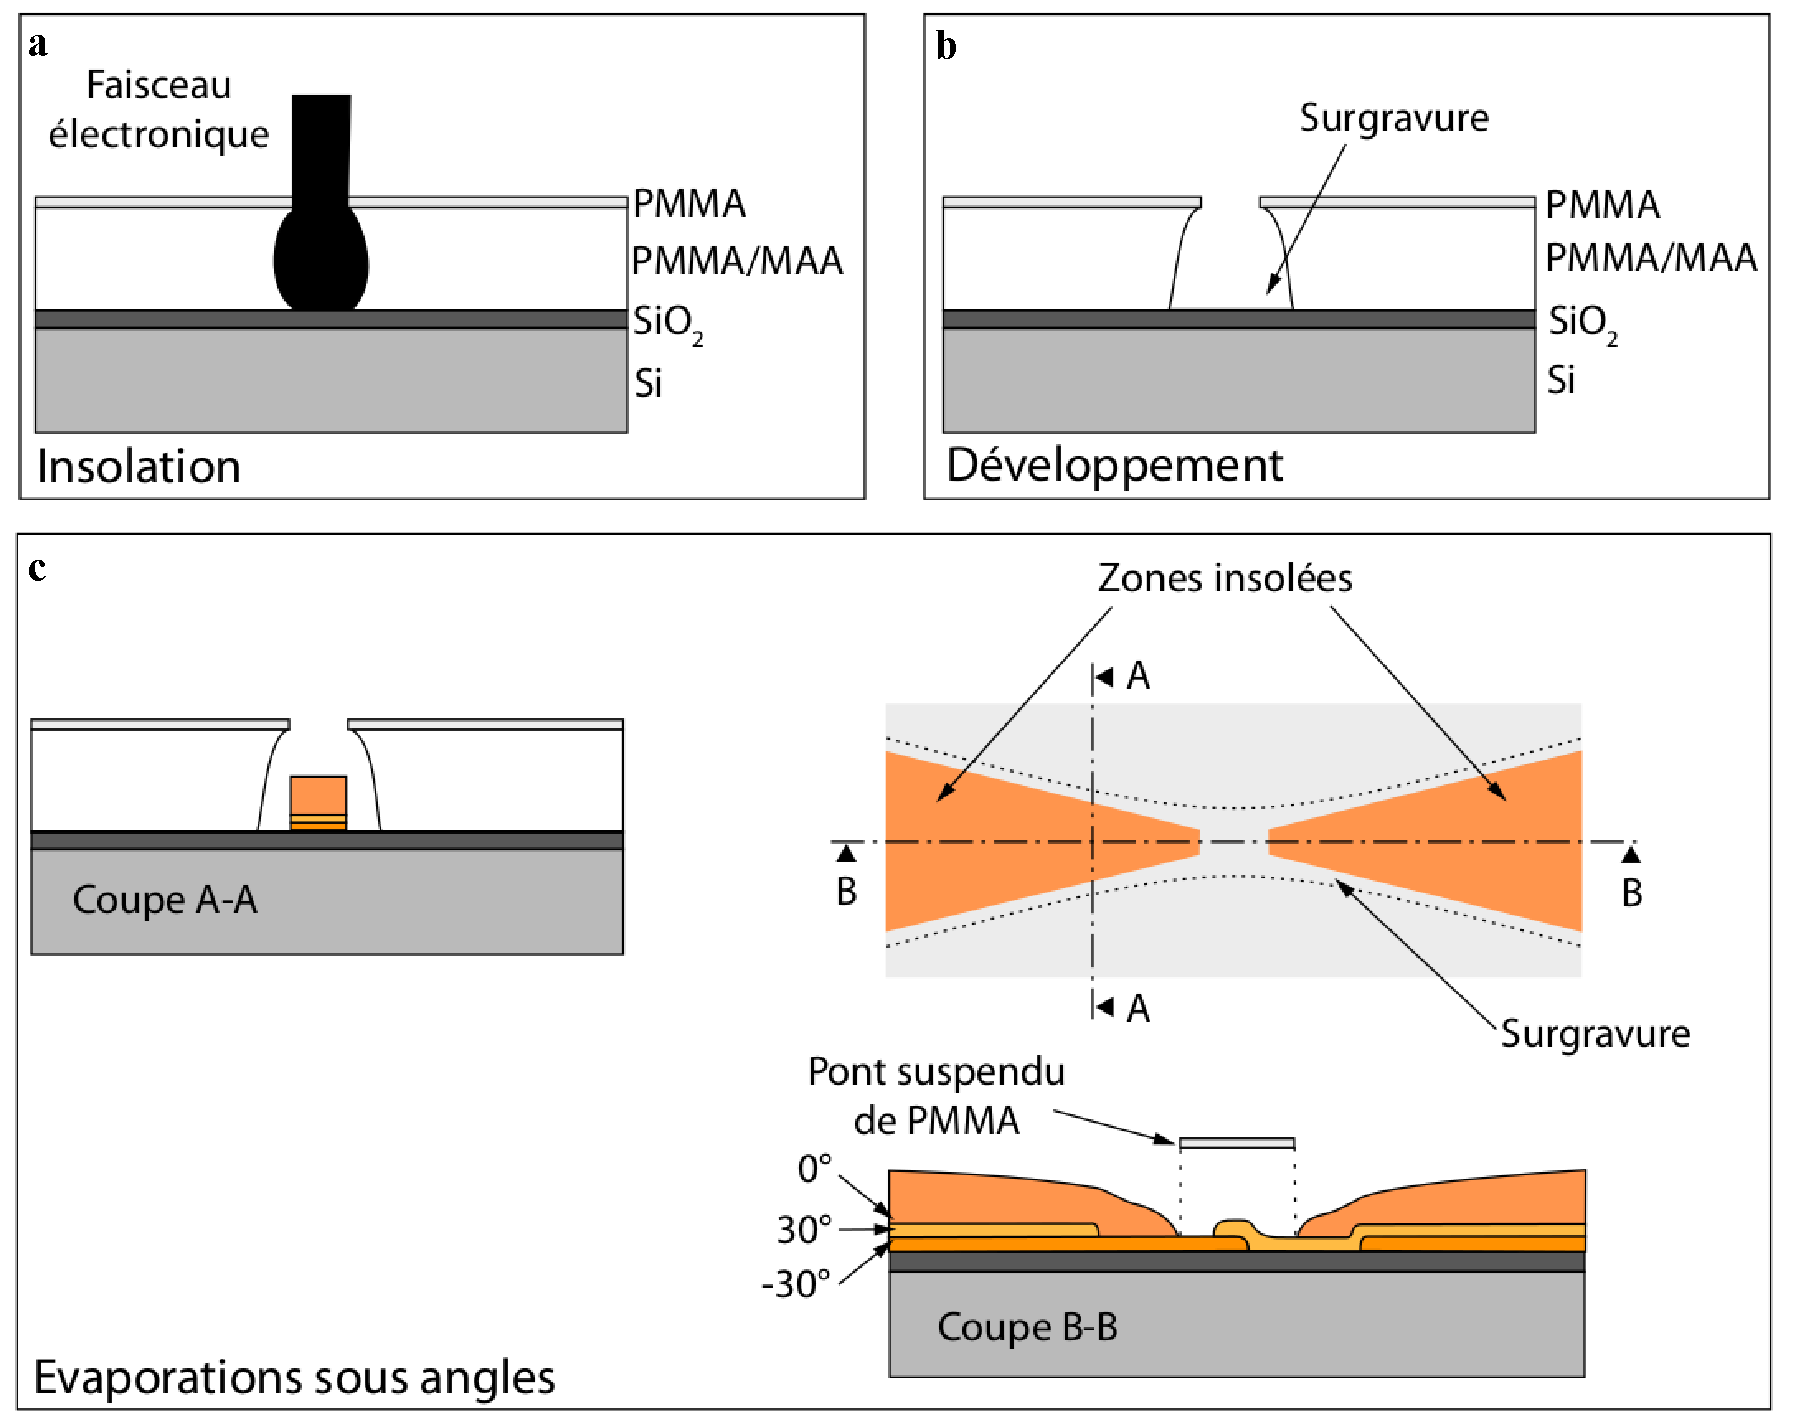
\includegraphics[scale=0.45]{Fabrication/EvapAngle/EvapAngle.pdf}
\caption{\textbf{a} : Insolation par lithographie électronique de la bicouche de résine. La partie la plus proche du substrat~(PMMA/MAA) se trouve plus insolée de par une plus grande sensibilité aux électrons et la présence des électrons rétrodiffusés. \textbf{b} : résultats après développement montrant clairement la surgravure générée par la surexposition de la partie basse. \textbf{c} : Evaporation sous angles : différentes couleurs représentent les différents angles d'évaporation (-30$\,\degres$, 0$\,\degres$ et 30$\,\degres$ - extrait de \cite{RochPhD}).}
\label{EvapAngle}
\end{figure}

Le nanofil va également avoir un impact sur le couplage de la molécule à la grille. Cette dépendance se fait de deux manières. Tout d'abord, la forme de pointe, donnée au niveau de la partie fine du nanofil, va minimiser l'écrantage une fois le gap obtenu. Une analyse des différents paramètres influençant cet écrantage est disponible dans~\cite{Datta2009}. Ensuite, en ayant une largeur faible, la surface en vis-à-vis avec la grille, et donc le risque de fuite de grille à travers un défaut de l'oxyde, est minimisée, augmentant la tension maximale applicable.

\begin{table}
\begin{center}
\begin{tabular}{|p{0.5cm}|p{4cm}|p{4cm}|p{3cm}|}
  \hline
\,& \textbf{étape} & \textbf{procédé} & \textbf{paramètres} \tabularnewline
\hline
1 &  dép\^ot de résine PMMA/MMA 2\,\% en masse & tournette & v\,:\,$6000\,$tr.min$^{-1}$, a\,:\,$4000\,$tr.min$^{-2}$, t\,:\,$30\,$s 
\tabularnewline
\hline
 2 & recuit (softbake) & plaque chauffante  & 5 minutes à 200$\, \degres C$ 
\tabularnewline
\hline
 3 & dépôt de résine PMMA 33\% en masse & tournette & v\,:\,$1400\,$tr.min$^{-1}$, a\,:\,$2000\,$tr.min$^{-2}$, t\,:\,$30\,$s \tabularnewline
\hline
4 & recuit & plaque chauffante & 5 minutes à 180$\, \degres C$
\tabularnewline
\hline
5 & insolation & MEB & dose de 240\,$\mu C.cm^{-2}$
\tabularnewline
\hline
6 & développement & becher MIBK/IPA ($1:3$) & 30 secondes
\tabularnewline
\hline
7 & rinçage & bécher IPA & 2 secondes
\tabularnewline
\hline
8 & surdéveloppement & bécher IPA & 1\,minute
\tabularnewline
\hline
9 & neutralisation du développeur &bécher d'eau désionisée & $1\,$minute\tabularnewline
\hline
10 & dép\^ot de la couche d'accroche & évaporateur à canon à électron PLASSYS & $3\,$nm de Ti à $0.05\,$nm.s$^{-1}$, angle=$0\,\degres$
\tabularnewline
\hline
11 & dépôt de la constriction & évaporateur à canon à électron PLASSYS & $10\,$nm de Au à $0.03\,$nm.s$^{-1}$, angle=$\pm 30\degres$
\tabularnewline
\hline
12 &  dépôt des nanofils &  évaporateur à canon à électron PLASSYS  &  $80\,$nm de Au à $0.15\,$nm.s$^{-1}$, angle=$\pm 0\degres$
\tabularnewline
\hline
 13 & lift-off & bécher d'acétone & 1\,heure minimum 
\tabularnewline
\hline
14 & rinçage & acétone, éthanol et isopropanol & 
\tabularnewline
\hline
15 & séchage & azote sec & 
\tabularnewline
\hline
16 & nettoyage & plasma oxygène (RIE)& $3\,$min\tabularnewline
\hline
\end{tabular}
\caption{Recette du bicouche PMMA/MAA : celle-ci permet d'obtenir des constrictions idéales pour l'électromigration.}
\label{tab_recette_elec}
\end{center}
\end{table}


Afin d'obtenir des fils répondant à ces critères, nous avons utilisé une méthode dite d'évaporation sous angles. Pour cela, il faut tout d'abord déposer deux couches de résine, la partie supérieure étant constituée de PMMA et la partie inférieure de PMMA-MAA, plus sensible aux électrons~(cf Fig.\ref{EvapAngle}). On procède ensuite à la lithographie électronique puis au développement de la résine en suivant la recette du Tab.\ref{tab_recette_elec}. Du fait de la plus grande sensibilité de la partie inférieure et la présence d'électrons rétrodiffusés, on obtient une partie sur-insolée entraînant la formation d'un ``pont" comme décrit sur la Fig.\ref{EvapAngle}.

On évapore ensuite une fine couche de titane~(3$\, nm$) avec un angle de $0\,\degres$ pour constituer un couche d'accroche, puis sous un angle de $\pm30\,\degres$, $10\, nm$ d'or  constituant la constriction. Enfin, $80\,nm$ d'or sont évaporés à $0\,\degres$ afin de venir relier la constriction aux plots de connexion. Cette épaisseur doit être suffisante pour assurer un bon passage entre la partie se situant sur la grille et celle se trouvant sur la surface même du wafer. La structure finale est présentée dans la Fig.\ref{FinalResult}.\textbf{b} et \textbf{c}.


\section{Réalisation d'un interstice nanométrique}
Une fois obtenues nos constrictions métalliques, il faut procéder à la dernière étape de fabrication : l'électromigration. Celle-ci, effectuée à une température de $4\,K$, va nous permettre d'obtenir les interstices de quelques nanomètres de largeur, nécessaires à la fabrication d'un transistor moléculaire. Dans ce chapitre, nous présenterons dans un premier temps la technique d'électromigration ainsi que les différentes méthodes de mise en œuvre. Nous finirons par une description de notre technique de contre-réaction rapide à basse température.

\subsection{L'électromigration}
L'électromigration est un phénomène connu depuis plus d'un siècle maintenant~\cite{Gerardin1861}. Ce phénomène a connu un regain d'intérêt avec le développement de la micro-électronique, notamment parce qu'il a été identifié comme étant une cause de panne récurrente~\cite{Blech1967,Black1969}.
Il se produit lorsqu'une forte densité de courant traverse un conducteur. Les ions du réseau sont alors soumis à deux forces : la première est induite par le champ électrique générant le courant, la seconde est due aux électrons qui, du fait de la diffusion, viennent céder un peu de leur moment cinétique aux ions du réseau~\cite{Ho1989}. L'action de ces deux forces se résume par la formule suivante :
\begin{eqnarray}
\textbf{F} = \textbf{F}_d + \textbf{F}_v = Z^*e\textbf{E} \nonumber
\end{eqnarray}
où $\textbf{F}_d$ est la force induite par le champ électrique et $\textbf{F}_v$ celle induite par la diffusion des électrons. Le terme $Z^*$ est en général utilisé pour représenter la charge effective des ions soumis à un champ électrique, et rend compte de l'interaction ions/électrons.

Ce phénomène a été pour la première fois utilisé en électronique moléculaire par le groupe de D.C. Ralph à Cornell~\cite{Park1999}. La technique a notamment été mis en oeuvre pour réaliser le premier transistor à molécule unique~\cite{Park2000}. Depuis, elle a connu de nombreuses évolutions comme nous allons le voir maintenant

\subsection{Etat de l'art}
On peut classer les techniques d'électromigrations en trois grandes catégories : à rampe unique, à contre-réaction et à cassure-spontanée. Une analyse plus fine des différentes méthodes est disponible dans~\cite{Girod2012}.

\subsubsection{À rampe unique}
C'est la première technique a avoir été mise en œuvre dans le domaine de l'électronique moléculaire par Park \textit{et al.}~\cite{Park1999}. Elle consiste en l'application d'une rampe de tension croissante sur un fin fil de métal (voir Fig.\ref{ParkExemp}). La simplicité de la méthode est séduisante, mais mal contrôlée, elle peut conduire à une destruction de la jonction, notamment due au chauffage induit par effet Joule.

\begin{figure}
\parbox{7cm}{
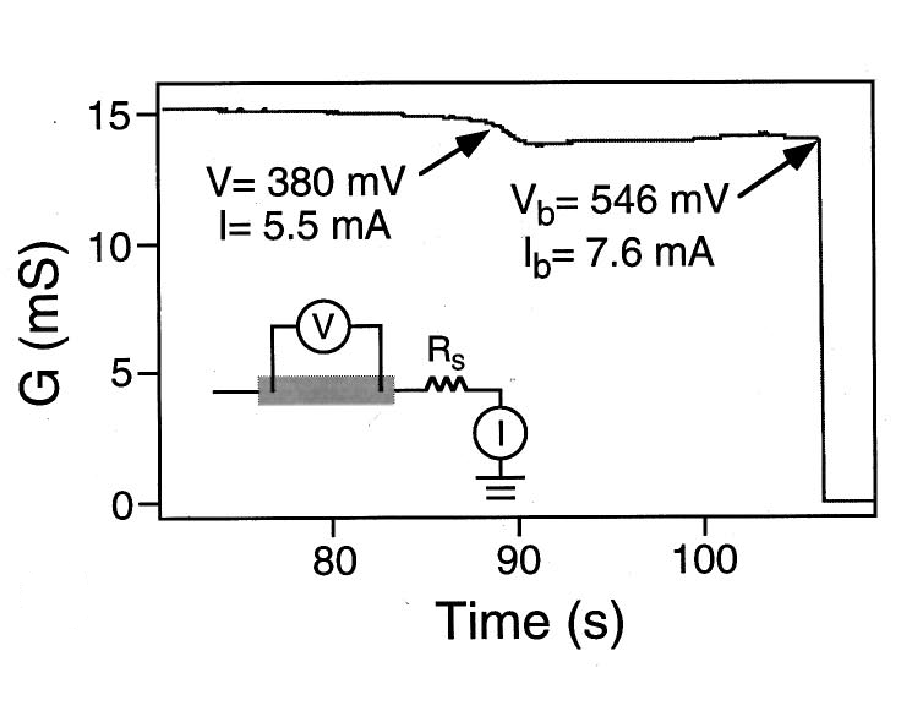
\includegraphics[scale=0.45]{Fabrication/ElecMigExemp/ParkFig.pdf} 
}
\parbox{6.5cm}{\caption{Evolution de la conductance d'un nanofil au court du temps lors d'une procédure d'électromigration à rampe unique. Extrait de~\cite{Park1999}.}
\label{ParkExemp}
}
\end{figure}



\subsubsection{À contre-réaction}
Cette méthode à été développée par Strachan \textit{et al.} en 2005~\cite{Strachan2005}. Elle a pour but de réduire le chauffage de la jonction par effet Joule~\cite{Esen2005} en introduisant une boucle de contre-réaction asservie sur la résistance de la jonction. Si celle-ci dépasse une valeur critique fixée à l'avance, la tension est diminuée puis augmente à nouveau. Ceci a pour effet de réduire la puissance dissipée par la jonction lors de l'électromigration (voir Fig.\ref{EseExemp}). Le principal inconvénient de cette technique est son temps de mise en œuvre : la formation d'un seul gap peut prendre plusieurs heures.


\begin{figure}
\parbox{7cm}{
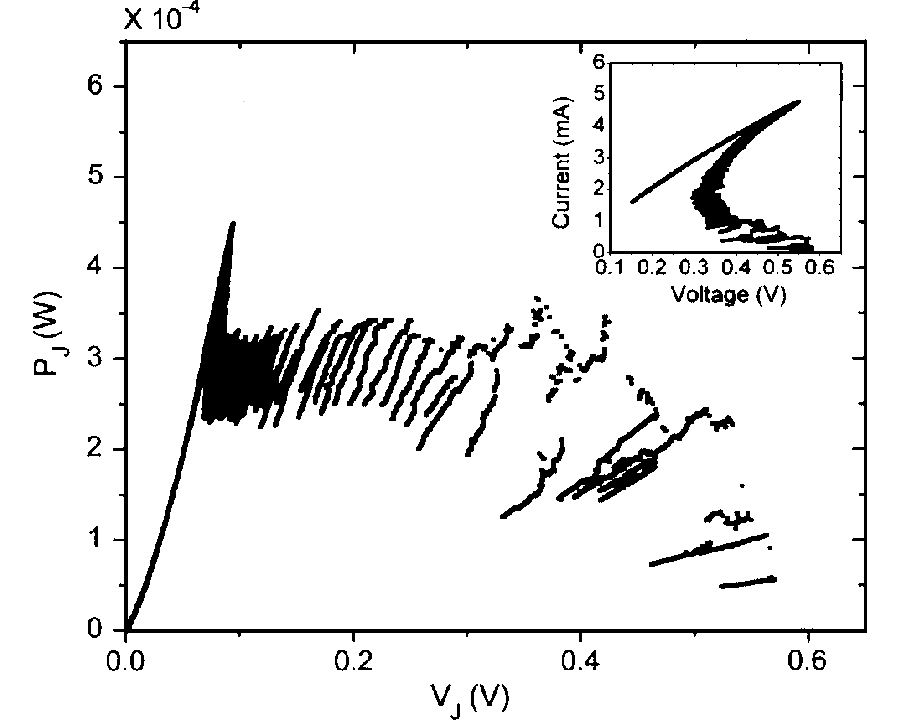
\includegraphics[scale=0.45]{Fabrication/ElecMigExemp/EseFig.pdf} 
}
\parbox{6.5cm}{\caption{Evolution de la puissance dissipée en fonction de la tension appliquée, lors d'une procédure d'électromigration à contre-réaction. En encart, caractéristique courant-tension lors de cette m\^eme procédure. Extrait de~\cite{Esen2005}.}
\label{EseExemp}
}
\end{figure}


\subsubsection{À cassure spontanée}

\begin{figure}
\parbox{7cm}{
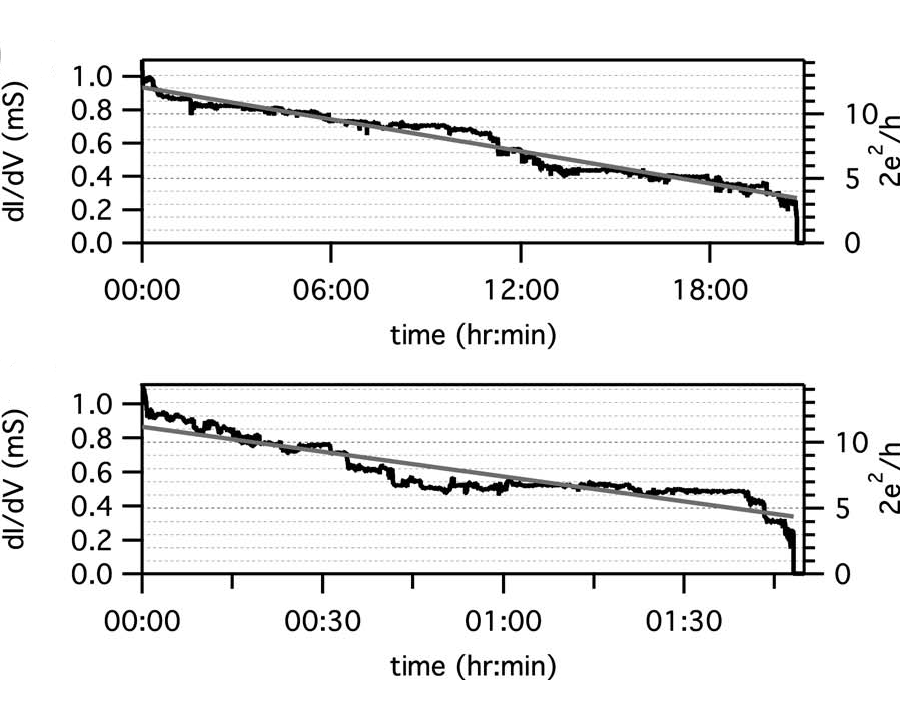
\includegraphics[scale=0.45]{Fabrication/ElecMigExemp/ZantFig.pdf} 
}
\parbox{6.5cm}{\caption{Évolution de la conductance de deux nanofils au cours du temps lors d'une procédure d'électromigration à cassure spontanée. Extrait de~\cite{ONeill2007}.}
\label{ZantExemp}
}
\end{figure}
Cette dernière méthode a été mise au point dans le groupe de H.S.J. van der Zant en 2007~\cite{ONeill2007}. Une première étape d'électromigration contrôlée est d'abord réalisée, à température ambiante, à l'aide d'une méthode à contre-réaction jusqu'à ce que la conductance du nanofil atteigne une valeur de quelques kilo-Ohms. On laisse ensuite évoluer la jonction qui, du fait de l'instabilité de la nanoconstriction, va se rompre naturellement. On obtient ainsi un gap de quelques nanomètres. La durée d'une telle procédure varie d'un échantillon à l'autre : de quelques minutes à plusieurs heures (voir Fig.\ref{ZantExemp}).


\subsection{Notre technique}


\begin{figure}
\centering 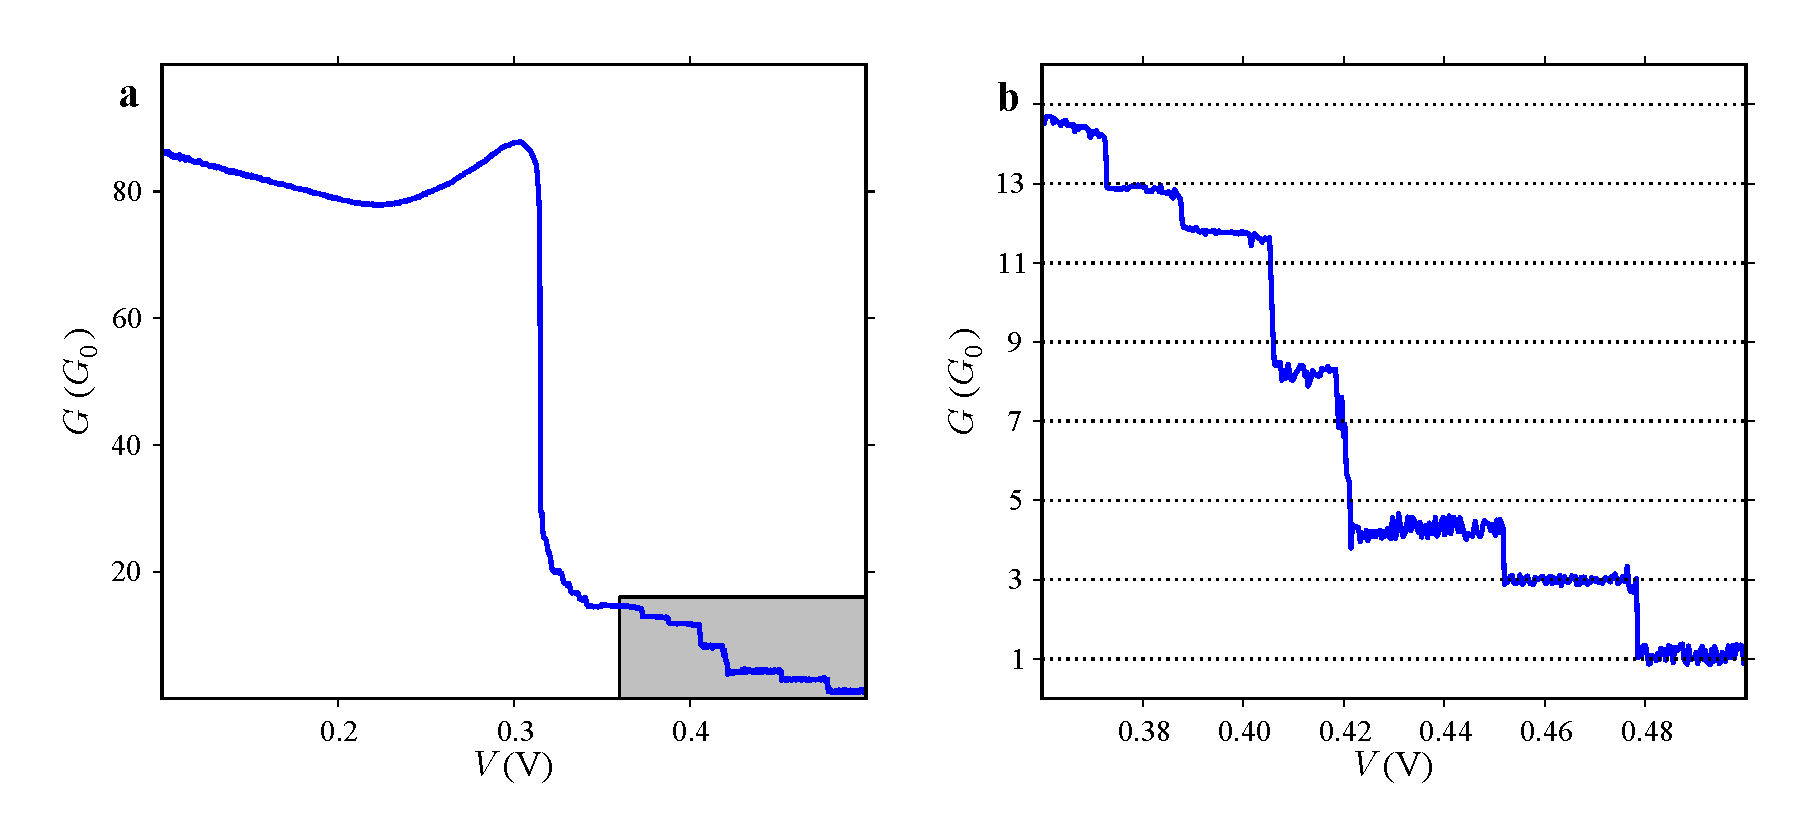
\includegraphics[scale=0.45]{Fabrication/NotreElectroMig/NotreElectroMig.pdf}
\caption{\textbf{a} : conductance de la jonction durant l'électromigration. \textbf{b} : grossissement de la partie grisée de \textbf{a} montrant les marches de conductance témoignant du bon déroulement de l'électromigration.}
\label{NotreElecMig}
\end{figure}

Notre technique de fabrication a été développée à partir des travaux de Park \textit{et al.}~\cite{Park1999} puis améliorée en s'inspirant de travaux ultérieurs.
Afin d'augmenter le rendement de la méthode et la qualité des interstices obtenus, il a fallu apporter quelques modifications. De plus, celle-ci étant réalisée dans un réfrigérateur à dilution, il a fallu adapter la procédure à l'impédance des lignes, induite par les différents étages de filtrage, en essayant de conserver celle-ci aussi basse que possible~(150\,$\Omega$). En effet, une faible impédance permet de limiter la puissance dissipée au niveau de la jonction et donc de mieux contrôler l'électromigration~\cite{Zant2006,Trouwborst2006,Taychatanapat2007}.

La présence de cette impédance nous impose de contrôler parfaitement le déroulement de l'électromigration. Pour cela, il faut être capable d'agir sur cette dernière en un intervalle de temps similaire à l'échelle de temps du phénomène : du domaine de la centaine de $\mu s$~\cite{ONeill2007}. Ceci n'est possible que si la procédure d'électromigration se fait à l'aide d'une électronique en temps réel. Nous avons pour cela utilisé un ADWin contrôlé par le programme NanoQT, développé au sein du groupe. Grâce à ce dispositif, l'électromigration peut être détectée et la tension aux bornes de la jonction ramenée à zéro dans un intervalle de $10\, \mu s$. Ainsi, nous pouvons obtenir des interstices de la taille souhaitée ($\sim 1\,nm$) de façon reproductible. 



\begin{figure}
\parbox{7cm}{
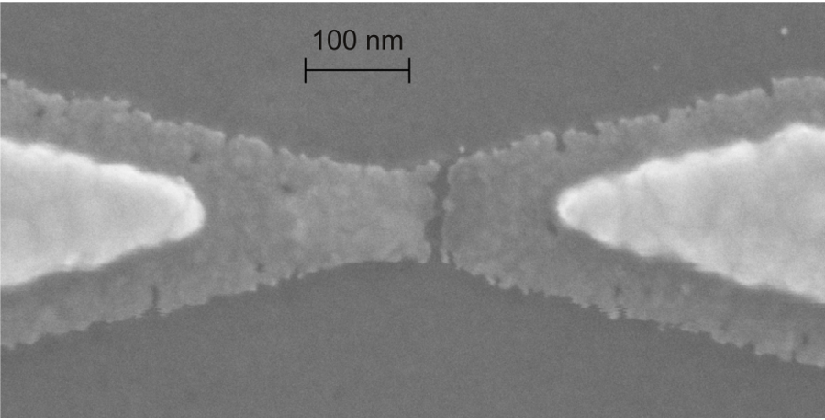
\includegraphics[scale=0.45]{Fabrication/JonctionElecromig/JonctionElecromig.pdf} 
}
\parbox{5cm}{\caption{Image obtenue par microscopie électronique à balayage d'une jonction électromigrée pour laquelle l'interstice nanométrique est clairement visible.}
}
\end{figure}


La Fig.\ref{NotreElecMig} présente la mesure en conductance lors d'un procédure d'électromigration. On observe trois régimes : dans un premier temps, la conductance diminue du fait de l'effet Joule; puis celle-ci augmente à nouveau du fait d'un réarangement de la jonction; enfin, la conductance chute brutalement et le phénomène d'électromigration commence. On peut notamment observer, en fin de procédure, une quantification de la conductance matérialisée par des plateaux, démontrant que l'électromigration est parfaitement contrôlée.

De plus, l'étape d'électromigration se fait à $4\,K$ et sous atmosphère d'hélium ce qui prévient la contamination de l'interstice et permet d'analyser le dispositif obtenu directement après la procédure.

\section{Fabrication d'un transistor à molécule unique}
Les étapes que nous avons présentées jusqu'à maintenant permettent d'obtenir une structure à trois terminaux~(source, drain et grille). Il nous faut maintenant disposer une molécule unique dans cette structure afin d'obtenir un transistor moléculaire. Pour cela, nous verrons tout d'abord comment les molécules sont déposées avant électromigration. Cette dernière étant effectuée à $4\,K$, elle autorise une caractérisation électrique immédiatement après. Nous détaillerons cette dernière afin de voir quels indices trahissent la présence d'un objet dans l'interstice nanométrique.

Les cristaux de TbPc$_{2}$ sont dissous dans du dichlorométhane à la concentration 10$^{-6}mol.L^{-1}$. La solution obtenue est soumise à un bain d'ultrason afin de prévenir la formation d'agrégats. La présence de ces dernières pourrait interférer avec l'électromigration, empêchant les molécules de se faire piéger dans l'interstice. Une goutte de la solution obtenue est ensuite déposée sur l'échantillon et séchée par un flux d'azote. L'échantillon obtenu est ensuite microsoudé sur le porte échantillon, disposé dans un frigo à dilution et électromigré à une température de  $4\,K$. Les jonctions obtenues (jusqu'à 12 par échantillons) sont ensuite analysées en transport.

Une fois la jonction électromigrée, il faut s'assurer que l'interstice obtenue contienne un objet. La première analyse généralement effectuée consiste à mesurer la conductance du système en fonction de la tension de grille, pour une tension source-drain nulle. La présence d'un objet nanométrique fait apparaître un ou plusieurs pics, que l'on nomme pics de Coulomb~\cite{Beenakker1991,Wiel2002,Hanson2007}~(cf annexe sur le transport mésoscopique). 

Mais il faut aussi s'intéresser à la nature de l'objet piégé et s'assurer qu'il s'agit bien de la molécule déposée. C'est une question cruciale dans le domaine de l'électronique moléculaire, et en particulier lorsque l'on utilise la technique d'électromigration. En effet, de nombreuses configurations peuvent donner une signature en transport plus ou moins similaire. Une boite quantique peut \^etre formée par une bille d'or crée lors de l'électromigration, par un élement polluant introduit lors de la fabrication ou du dép\^ot des molécules, ou bien encore par la molécule que l'on chercherait à étudier. C'est à ce dernier cas que l'on souhaite s'intéresser.

Dans notre cas, nous connaissons la signature magnétique de la molécule que nous souhaitons étudier. Cela facilite considérablement l'interprétation de la mesure. Nous n'avons qu'à analyser les propriétés magnétiques de l'objet piégé au sein de l'interstice, pour en déduire la nature et la configuration en transport. La méthode utilisée sera détaillée dans le chapitre suivant, consacré aux résultats expérimentaux.  S'il s'avère que la molécule est bien responsable du transport électronique, alors nous avons obtenu un transistor moléculaire tel que celui décrit dans la Fig.\ref{ImageTrans}.


